\documentclass[a4paper]{article}

\usepackage{array}
\usepackage{placeins}
\usepackage{listings}
\usepackage{hyperref}
\usepackage{enumitem}
\usepackage{todonotes}

\usepackage{hopsantut}

\begin{document}
\maketitle{Optimizing Models With modeFRONTIER}

%\section*{Legal Notice}
%modeFRONTIER is the property of ESTECO SpA. Hopsan development team is not affiliated with modeFRONTIER.

\section*{Introduction}
This tutorial will demonstrate how to run Hopsan simulations from modeFRONTIER\footnote{modeFRONTIER is the property of ESTECO SpA. The Hopsan developers are not affiliated with modeFRONTIER or ESTECO SpA.}, a multi-objective optimization environment. This makes it possible to use powerful optimization algorithms and data analysis tools on a Hopsan model. It is also possible to connect other programs to modeFRONTIER simultaneously and run multi-disciplinary optimizations. This is, however, not covered by this tutorial.

\section*{Requirements}
In this tutorial modeFRONTIER version 4.5.3 and Hopsan version 0.6.8 on a Windows operating system are used. It should, however, work on Linux systems with some minor modifications. Some basic knowledge of Hopsan and design optimization is also required. It is recommended to do the "Getting Started", "Advanced Usage" and "Optimization" tutorials before this one.
%\icon{0}{gfx/Hopsan-ExportSimulink.png}{Export model to Simulink S-function}

\section*{Optimize using final values only}
An optimization basically consists of three parts: A simulation model, one or more objective function(s), and an optimization algorithm. In this case Hopsan will be responsible for the simulation, while modeFRONTIER will take care of the algorithm. The evaluation of the objective function(s) can, however, be placed in either one of the programs. We will demonstrate both methods.

Calculating objective function values requires access to the resulting data variables from the simulation. Letting Hopsan do the calculation can therefore be easier, since the amount of data that must be send between the programs can be reduced. We will first show how to run an optimization by only sending the final simulation values from Hopsan.

\begin{tutenumerate}
\tutitem{Preparations}
For this example we will use the position servo example model. The objective is to optimize the parameters of the PI-controller by analyzing a step response. First we must modify the model so that it also calculates the objective function value.

\begin{itemize}
\item Open the position servo example
\item Add an absolute value operaetor and an integrator
\item Connect them after the error signal and name the integrator "totalError"
\item Create a new empty folder
\item Save the model as "PositionServo.hmf" in the folder you created
\end{itemize}

It should now look similar to the picture below:

\begin{center}
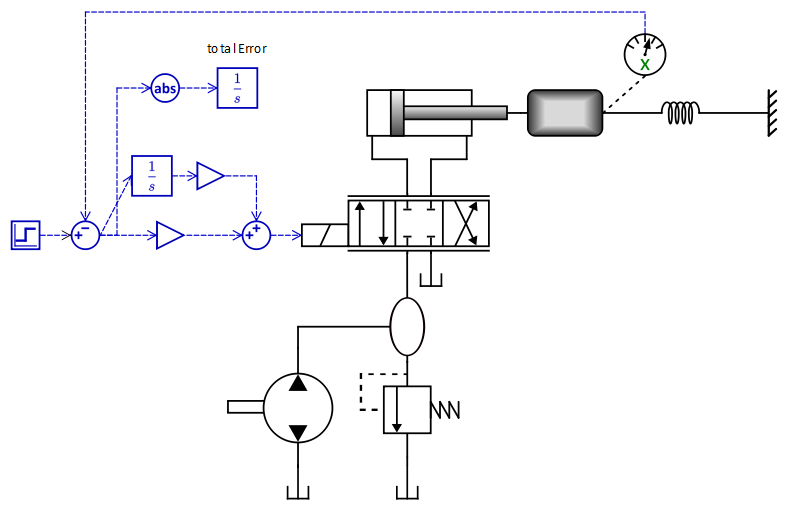
\includegraphics[width=0.7\textwidth]{gfx/modefrontier/hopsanmodel.png}\\
\end{center}

Hopsan and modeFRONTIER will communicate by using comma-separated files (.csv). Before we create the modeFRONTIER project we will need to extract two files from Hopsan to use as templates.
\begin{itemize}
\item Open a command prompt in Windows
\item Go to the folder you created
\item Execute HopsanCLI with the following command (change the Hopsan installation path to the one you have):
\begin{lstlisting}[basicstyle=\ttfamily\footnotesize, breaklines=true]
c:\"Program Files (x86)"\hopsan\bin\HopsanCLI --hmf PositionServo.hmf    --simulate hmf --resultsFinalCSV resultsFinal.csv 
    --parameterExport parameters.csv
\end{lstlisting}
\end{itemize}

This will open the model, simulate it and generate .csv files for parameters and final values of the data variables.


\tutitem{Build the modeFRONTIER project}
Now it is time to build the project in modeFRONTIER.

\begin{itemize}
\item Open modeFRONTIER
\item Create a new project and save it in the folder you created
\item Add the following process nodes:
\begin{itemize}
\item Scheduler
\item DOS Batch Script
\item Logic End
\end{itemize}
\item Add the following nodes for input data:
\begin{itemize}
\item 2x Input Variable
\item Input File
\item Support File
\end{itemize}
\item Add the following nodes for output data:
\begin{itemize}
\item Output File
\item Output Variable
\item Design Objective
\end{itemize}
\item Connect the nodes as shown in the picture below
\begin{center}
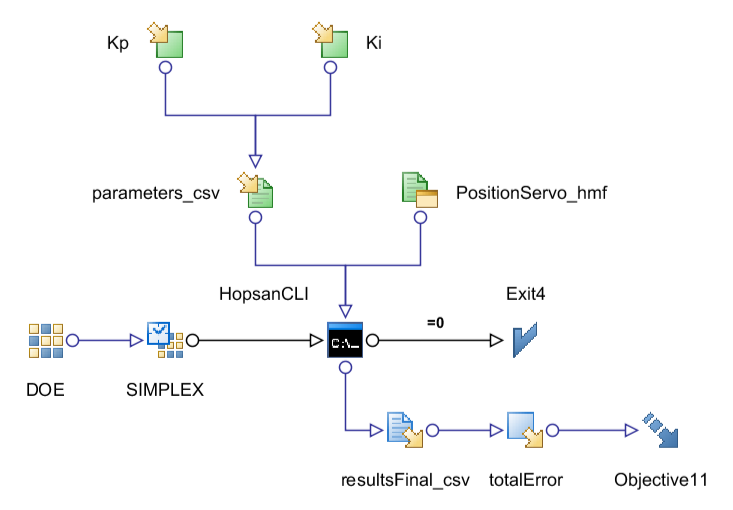
\includegraphics[scale=0.52]{gfx/modefrontier/model_final.png}\\
\end{center}
\end{itemize}


\tutitem{Specify input variables}
We will use two input variables, one for the proportional gain ($Kp$) and one for the integrating gain ($Ki$) in the PI controller.
\begin{itemize}
\item Double-click on one of the input variable nodes

\icon{0}{gfx/modefrontier/input_variable.png}{Input Variable}

\item Change \textit{"Name"} to \textit{"Kp"}
\item Set \textit{"Lower Bound"} to 0.0 and \textit{"Upper Bound"} to 0.01
\item Double-click on the second input variable node
\item Change name to \textit{"Ki"}, lower bound to 0.0 and upper bound to 0.005
\end{itemize}

\tutitem{Configure the input variable file}
Input variables shall be written to the "\texttt{parameters.csv}" file by modeFRONTIER, which is in turn loaded by Hopsan.
\begin{itemize}
\item Double-click on the input file node

\icon{0}{gfx/modefrontier/input_file.png}{Input File}
\item Set \textit{"Input File Node Name"} to \textit{"parameters\_csv"}
\item Click on \textit{"Edit Input File"}
\item Browse to the your folder and select "\texttt{parameters.csv}"
\item Select \textit{"Kp"} in the list at the bottom
\item Find the row that begins with \textit{"PositionServo\$GainP\#k\#Value"}
\item Select the numerical value at the end of the row
\item Right-click and choose \textit{"Insert Variable"}
\item Select \textit{"Ki"} in the list at the bottom
\item Find the row that begins with \textit{"PositionServo\$GainI\#k\#Value"}
\item Select the numerical value at the end of the row
\item Right-click and choose \textit{"Insert Variable"}
\item Click \textit{"Ok"} twice to close the dialogs
\end{itemize}

\tutitem{Configure the Hopsan model file}
We must also specify the model file used by Hopsan.
\begin{itemize}
\item Double-click on the support file node

\icon{0}{gfx/modefrontier/support_file.png}{Support File}

\item Set \textit{"Support File Node Name"} to \textit{"PositionServo\_hmf"}
\item Click on \textit{"Add File"} and select "\texttt{PositionServo.hmf}"
\item Click \textit{"Ok"}
\end{itemize}

\tutitem{Specify the output variable}
The output variable consist of the integrated error signal from the Hopsan model.
\begin{itemize}
\item Double-click on the output variable node

\icon{0}{gfx/modefrontier/output_variable.png}{Output Variable}

\item Set \textit{"Name"} to \textit{"totalError"}
\item Click \textit{"Ok"}
\end{itemize}

\tutitem{Configure the output file}
The output value is read by modeFRONTIER from "\texttt{resultsFinal.csv}", which contains the final values exported from Hopsan.
\begin{itemize}
\item Double-click on the output file node

\icon{0}{gfx/modefrontier/output_file.png}{Output File}

\item Set \textit{"Output File Node Name"} to \textit{"resultsFinal\_csv"}
\item Click on \textit{"Open Output File"}
\item Select "\texttt{resultsFinal.csv}"
\item Find the row that starts with \textit{"PositionServo\$totalError\#out\#Value"}
\item Select \textit{"totalError"} at the bottom
\item Select the text \textit{"PositionServo\$totalError\#out\#Value"}
\item Right-click and choose \textit{"Select Relative"}
\item Click \textit{"Ok"} twice
\end{itemize}

\tutitem{Define the objective function}
The objective function in modeFRONTIER will be to simply minimize the value obtained from Hopsan.
\begin{itemize}
\item Double-click on the design objective node

\icon{0}{gfx/modefrontier/design_objective.png}{Design Objective}

\item Change from \textit{"Maximize"} to \textit{"Minimize"}
\item Click \textit{"Ok"}
\end{itemize}

\pagebreak

\tutitem{Write a script for controlling HopsanCLI}
Hopsan will be controlled through the command line interface (\texttt{HopsanCLI.exe}) from a batch script in modeFRONTIER.
\begin{itemize}
\item Double-click on the script node

\icon{0}{gfx/modefrontier/dos_batch_script.png}{DOS Batch Script}

\item Set \textit{"Name"} to \textit{"HopsanCLI"}
\item Click on \textit{"Edit DOS Batch Script"}
\item Enter the following command:
\begin{lstlisting}[basicstyle=\footnotesize\ttfamily, breaklines=true]
C:\"Program Files (x86)"\Hopsan\bin\HopsanCLI --hmf PositionServo.hmf
    --simulate hmf --resultsFinalCSV resultsFinal.csv 
    --parameterImport parameters.csv
\end{lstlisting}
This will tell HopsanCLI to load the specified model, load parameters from \texttt{parameters.csv}, simulate the model and then write the final values of all data variables to \texttt{resultsFinal.csv}.
\item Click \textit{"Ok"} twice
\end{itemize}

\tutitem{Choose initial distribution and algorithm}
Finally, we must configure the optimization in modeFRONTIER. For this example we will use a random initial distribution and the Simplex algorithm. It is of course possible to use other distributions and algorithms as well.
\begin{itemize}
\item Double-click on the DOE node

\icon{0}{gfx/modefrontier/doe}{DOE}

\item Select \textit{"Random"} under \textit{"Space Fillers"} to the left
\item Click on \textit{"Add DOE Sequence"}
\item Click \textit{"Ok"}
\item Double-click on the scheduler node

\icon{0}{gfx/modefrontier/scheduler.png}{Scheduler}

\item Select \textit{"Simplex"} under \textit{"Heuristic Optimizers"}
\item Click \textit{"Ok"}
\end{itemize}

\tutitem{Run an optimization}
Now everything is prepared for starting the optimization!
\begin{itemize}
\item Make sure the model is saved
\item Go to the \textit{"Run Analysis"} mode
\item Start the optimization by clicking on the green arrow to the top right of the workspace

\icon{0}{gfx/modefrontier/run_stop.png}{Run/Stop}

\end{itemize}
\end{enumerate}



\section*{Optimizing using full variable export}
Putting the objective function in Hopsan is not always possible (or desirable). Another method is to export the data to modeFRONTIER instead, so that the calculation can be made there.

\begin{enumerate}
\tutitem{Save a copy of the model}
Save the model from the previous section in the same folder but with a different name.

\tutitem{Generate output variable file}
First we need to generate a new .csv file to use as a template for the data.
\begin{itemize}
\item Open the command prompt in Windows and go to your folder
\item Start HopsanCLI with the following command:
\begin{lstlisting}[basicstyle=\footnotesize\ttfamily, breaklines=true]
c:\Program Files (x86)"\hopsan\bin\HopsanCLI --hmf PositionServo.hmf 
    --simulate hmf --resultsFinalCSV resultsFinal.csv  
\end{lstlisting}
\end{itemize}
This will generate a file called "\texttt{resultsFinal.csv}", which we will use below.

\tutitem{Modify the HopsanCLI script}
Now we must modify the script where modeFRONTIER calls HopsanCLI, so that the full result file is updated after each simulation.
\begin{itemize}
\item Double-click on the script node

\icon{0}{gfx/modefrontier/dos_batch_script.png}{DOS Batch Script}

\item Click on \textit{"Edit DOS Batch Script"}
\item Modify the command to the following:
\begin{lstlisting}[basicstyle=\footnotesize\ttfamily, breaklines=true]
C:\"Program Files (x86)"\Hopsan\bin\HopsanCLI --hmf PositionServo.hmf
    --simulate hmf --resultsFullCSV resultsFull.csv 
    --parameterImport parameters.csv
\end{lstlisting}
\item Click \textit{"Ok"} twice
\end{itemize}

\tutitem{Modify the project}
The project in modeFRONTIER must be modified, so that the objective function is calculated. 
\begin{itemize}
\item Remove the output file node (called \textit{"resultsFinal\_csv"})
\item Add an Output Template node and a Calculator node between the script and the exit nodes
\item Add a Transfer File node between the Script node and the Output Template node
\item Add two Output Vector nodes between the Output Template node and the Calculator node
\item Connect the calculator node with the existing \textit{"totalError"} node
\end{itemize}

The model should now look like this:

\begin{center}
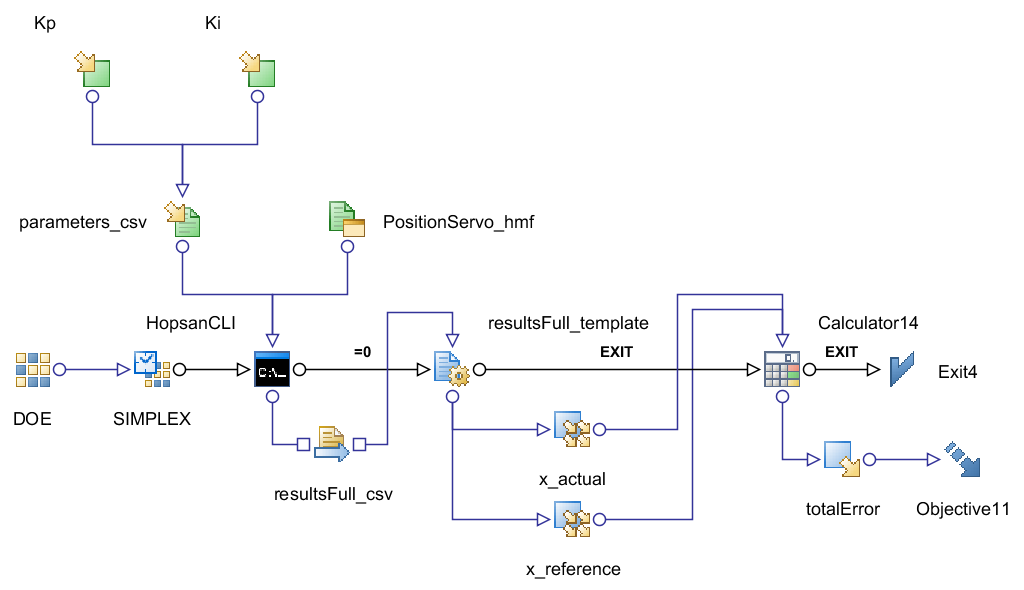
\includegraphics[scale=0.52]{gfx/modefrontier/model_full.png}
\end{center}


\tutitem{Specify output variables}
We will use two output variables from Hopsan, the reference piston position and the actual position.
\begin{itemize}
\item Double-click on one of the output vector nodes

\icon{0}{gfx/modefrontier/vector_output_variable.png}{Vector Output Variable}

\item Set \textit{"Name"} to \textit{"x\_actual"}
\item Set \textit{"Size"} to 2048
\item Click \textit{"Ok"}
\item Double-click on the second output vector node
\item Set \textit{"Name"} to \textit{"x\_reference"}
\item Set \textit{"Size"} to 2048
\item Click \textit{"Ok"}
\end{itemize}

\tutitem{Configure the output varible file}
The output variables must be obtained from the generated .csv file.
\begin{itemize}
\item Double-click on the transfer file node

\icon{0}{gfx/modefrontier/transfer_file.png}{Transfer File}

\item Set \textit{"Transfer File Node Name"} to \textit{"resultsFull\_csv"}
\item Click on \textit{"Add File"}
\item Browse to your folder and select "\texttt{resultsFull.csv}"
\item Click \textit{"Ok"} twice
\end{itemize}

\tutitem{Configure the data mining}
Now we must specify the data mining, to map each variable to a block in the .csv file.
\begin{itemize}
\item Double-click on the output template node

\icon{0}{gfx/modefrontier/output_template.png}{Output Template}

\item Set \textit{"Output Template Node Name"} to \textit{"resultsFull\_template"}
\item Click on \textit{"Edit Output Template"}
\item Browse to your folder and select "\texttt{resultsFull.csv}"
\item Click on \textit{"x\_actual"} at the bottom
\item Find the row that starts with \textit{"PositionServo\$Position\_Sensor\#out\#Value"}
\item Select the text, right-click and choose \textit{"Add Rule For"} \textrightarrow  \textit{"x\_actual"}
\item Select the text again, right-click and choose \textit{"Set Anchor"} \textrightarrow  \textit{"x\_actual"}
\item Uncheck column 1, 2, 3 and 4 to the left
\item Click on \textit{"x\_reference"} at the bottom
\item Find the row that starts with \textit{"PositionServo\$Step\#out\#Value"}
\item Select the text, right-click and choose \textit{"Add Rule For"} \textrightarrow  \textit{"x\_reference"}
\item Select the text again, right-click and choose \textit{"Set Anchor"} \textrightarrow  \textit{"x\_reference"}
\item Uncheck column 1, 2, 3 and 4 to the left
\item Click \textit{"Ok"} twice
\end{itemize}

\tutitem{Define the objective function calculation}
Finally, we must also specify the equation for the objective function.
\begin{itemize}

\item Double-click on the calculator node

\icon{0}{gfx/modefrontier/calculator.png}{Calculator}

\item Set \textit{"Name"} to \textit{"objective\_function"}
\item Click on \textit{"Edit Calculator Expression"}
\item Enter the following expression:
\begin{lstlisting}
totalError = sum(abs(subtract(x_actual,x_reference)))
\end{lstlisting}
\item Click \textit{"Ok"} twice to close the dialog
\end{itemize}
  
\tutitem{Save the model and run an optimization}
If everything was successful, the optimization should work and give reasonable results. This method should, however, be less time-efficient, due to the large amount of data being exchanged between the programs.
\end{tutenumerate}

\end{document}